%% =====================================================================
%% METHODS -- MACRO ROADMAP
%% ---------------------------------------------------------------------
%% What this Methods section must convey:
%%   The full signal path from pre-generated per-participant stereo WAV
%%   files through a dual-channel audio interface to the participant,
%%   into a live event log, and back out via a loopback recording that
%%   is decoded offline to recover trial-wise reaction times.
%%   Participant responses are captured as an audible click tone
%%   routed to the tactile channel, loopback-recorded alongside the
%%   played stimulus, and recovered post-hoc by cross-correlation
%%   against a click template. This procedure decouples response
%%   timing from operating-system event latency and lets reaction
%%   time be computed in the sample domain of the audio stream that
%%   reached the hardware.
%%
%% ARGUMENTATIVE CHAIN (subsection-level):
%%   [Sub 1] Apparatus: what hardware carried the stimuli and captured
%%           the responses.
%%     -->
%%   [Sub 2] Stimulus generation: how the per-trial 8 s stereo WAV
%%           was built, from the box-breathing voice guide to the
%%           FABIAN-spatialised looming noise to the Woojer tactile
%%           pulse, and how per-participant 6-block sequences were
%%           assembled under a Gellermann-inspired constrained
%%           randomisation.
%%     -->
%%   [Sub 3] Trial design: what the 408 trials in a session consisted
%%           of (2 parts x 6 blocks x 34 trials) and how respiratory
%%           phase, SOA, and noise type were counterbalanced.
%%     -->
%%   [Sub 4] Stimulus delivery and response capture: how sounddevice
%%           routed the two WAV channels to the Sennheiser headphones
%%           and the Woojer Strap, how mouse responses were echoed as
%%           a click tone onto the tactile channel, and how WASAPI
%%           loopback captured both outputs.
%%     -->
%%   [Sub 5] Reaction-time reconstruction: how the continuous loopback
%%           recordings and live event logs were decoded to recover
%%           per-trial cue onset, click onset, and RT, and how outcomes
%%           were labelled.
%%     -->
%%   [Sub 6] Peripersonal-space quantification: how SOAs were converted
%%           into looming-source distances, how audio-tactile
%%           facilitation was computed, and how the PPS boundary was
%%           defined.
%%     -->
%%   [Sub 7] Respiratory compliance and participants.
%%
%% STYLE: prose avoids em-dashes, superfluous parentheses, and
%% redundant colons. Every factual claim is cited (peer-reviewed
%% where available, otherwise manufacturer or software reference).
%% =====================================================================

\section{Materials and Methods}

\begin{figure}[ht]
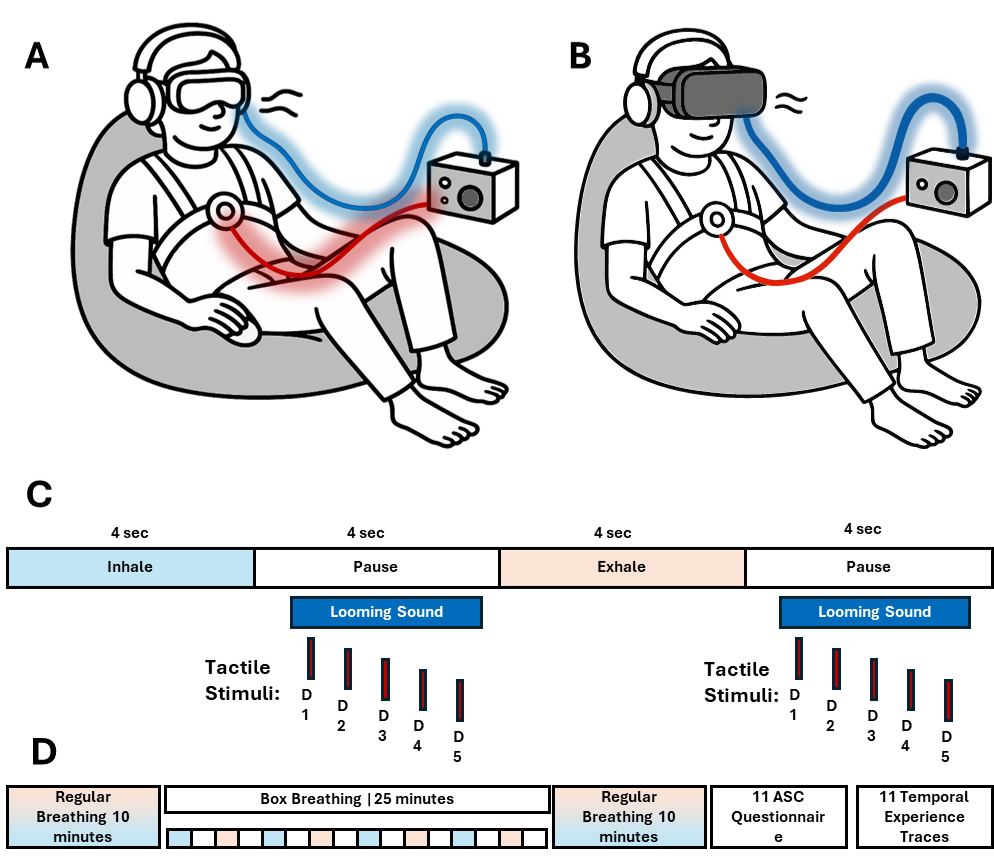
\includegraphics[width=\textwidth]{Fig1.png}
\caption{\textbf{Experimental setup and protocol.} \textbf{A}, Control condition setup with participant wearing headphones (blue cord) and a chest-mounted vibrotactile stimulator (red cord) positioned above the breast area as depicted on the strap itself, providing only the minimal breath-performance feedback indicator without spatial cues. \textbf{B}, Viscereality condition setup with the breath-responsive VR headset providing visual feedback of respiratory state. \textbf{C}, Box-breathing protocol with looming sounds and tactile stimuli presented during breath-hold phases. D1--D5 represent stimulus onset asynchronies between audio and tactile stimuli.}
\label{study5:fig:exp_setup}
\end{figure}

%% ---------------------------------------------------------------------
%% SUBSECTION 1 GOAL
%% One paragraph listing the hardware chain: soundcard, headphones,
%% haptic transducer, respiratory belt, response device, HMD. Ends
%% with the relationship between the two physical outputs of the
%% soundcard and the two transducers reaching the participant.
%% ---------------------------------------------------------------------
\subsection{Apparatus}

%% ---
%% PARAGRAPH GOAL (one idea): enumerate the hardware chain and fix
%% the two-channel output-to-transducer mapping that the rest of
%% the section depends on.
%% ---
Auditory and tactile stimuli were delivered through a Komplete Audio 6 MK2 USB audio interface \citep{komplete_audio_6_mk2}. The audio channel was routed to a pair of Sennheiser HD 560S open-back reference headphones \citep{sennheiser_hd560s}, worn over the ears, and the tactile channel was routed to a Woojer Strap 4 haptic transducer \citep{woojer_strap4}, worn over the chest just above the breast area. Placement was standardised across participants by following the positioning illustration printed on the strap itself, which the operator used as a fitting guide. Participant responses were collected with a standard USB mouse. Respiratory compliance was monitored throughout the session with a chest-mounted respiratory belt transducer positioned around the lower ribcage. In the Viscereality condition, participants additionally wore a head-mounted display delivering the breath-coupled visual environment. In the Control condition, participants viewed the same dark field used as the black-screen control in Study~3, containing only the central breathing performance indicator that scaled with respiratory excursion. This provided minimal feedback stimuli for breath performance without the spatial depth cues, color, or aesthetic properties of the Viscereality environment, and participants did not wear an eye shade (Fig.~\ref{study5:fig:exp_setup}).

%% ---------------------------------------------------------------------
%% SUBSECTION 2 GOAL
%% Describe how the per-participant stereo WAV files were built. Five
%% sub-blocks, one idea per paragraph:
%%   2a  Box-breathing voice guide (pre-recorded MP3).
%%   2b  Looming auditory stimulus (FABIAN HRTF spatialisation).
%%   2c  Tactile pulse (Woojer 4 spec).
%%   2d  Per-trial stereo WAV assembly.
%%   2e  Per-participant sequence construction.
%% ---------------------------------------------------------------------
\subsection{Stimulus generation}
\label{study5:sec:stim_gen}

%% ---
%% PARAGRAPH 2a GOAL (one idea): state that the box-breathing guide
%% is a pre-recorded human-voice MP3 (not a synthesised track), with
%% exact filename, resampling, volume, and channel placement. Keeps
%% the paragraph short and factual.
%% ---
The box-breathing guide was built from two pre-recorded human-voice audio files, one for the inhalation half-cycle and one for the exhalation half-cycle \citep{pydub_audiosegment_note}. Each file voiced a count of ``two, three, four, hold'' over four seconds so that a full 4--4--4--4 cycle of inhalation, post-inhalation hold, exhalation, and post-exhalation hold lasted sixteen seconds. Files were loaded at their source rate and resampled to 44.1~kHz using \texttt{librosa} where available and otherwise \texttt{scipy.signal.resample} \citep{Virtanen2020SciPy, librosa_resample_note}. Amplitude was attenuated to 30\% of source level so that the voice guide remained audible without masking the looming stimuli. The guide occupied the right channel of the per-trial stereo WAV, with the left channel set to silence over the same four-second span.

%% ---
%% PARAGRAPH 2b GOAL (one idea): describe the looming-sound pipeline
%% in enough detail that a reader could reproduce it. Emphasise the
%% FABIAN HRTF source (TU Berlin DepositOnce), the head-diameter and
%% inverse-square scaling, the four counterbalanced noise types,
%% the 110 to 10 cm frontal trajectory at 33.3 cm/s, and the
%% per-trial 500 ms silent padding that fixes the stimulus segment
%% to exactly 4 s.
%% ---
Binaural looming stimuli were initially synthesised from four noise types, namely pink, white, brown, and blue noise; later acquisition versions used a subset, predominantly pink and white \citep{brinkmann2017fabian}. For each noise type, a 3-second trajectory was rendered in which a point source approached the head frontally from 1.1~m to 0.1~m at a constant 33.3~cm/s, at zero azimuth and zero elevation. Source-to-ear distances were computed for an 18~cm interaural distance, and amplitude was scaled by the inverse square of source-to-ear distance. Head-related transfer function filtering used the measured FABIAN head-related impulse response at neutral head-above-torso orientation, specifically the \texttt{FABIAN\_HRIR\_measured\_HATO\_0.sofa} file from the FABIAN database hosted on the Technische Universit\"at Berlin DepositOnce repository \citep{fabian_database_2017, brinkmann2017fabian}. The SOFA file was parsed with the \texttt{sofar} Python library \citep{sofar_python}, the left and right impulse responses for the azimuth-zero, elevation-zero position were extracted, and each was convolved with the per-channel noise trajectory using \texttt{scipy.signal.fftconvolve} \citep{Virtanen2020SciPy}. Each looming file was normalised to 95\% of maximum amplitude to prevent digital clipping and was padded with 500~ms of silence before and after the 3-second approach, yielding a 4-second stimulus segment.

%% ---
%% PARAGRAPH 2c GOAL (one idea): specify the tactile pulse used for
%% the Woojer Strap 4 transducer. The current generator selects a
%% 50 Hz pure sine at amplitude 1.0 with an instant on/off block
%% envelope for 100 ms, so calibration is tuned to transducer
%% resonance rather than to perceptual thresholding.
%% ---
Tactile pulses were generated for the Woojer Strap 4 transducer, whose resonance is near 50~Hz. Each pulse was a 100~ms pure-tone 50~Hz sine at digital amplitude 1.0 with an instant-on, instant-off block envelope, chosen to deliver the maximum mechanical impulse the transducer supports \citep{woojer_strap4}. The stimulus-generation scripts can instantiate pulses at 0, 300, 800, 1500, 2200, and 2700~ms after looming onset, with the 0~ms file serving as an audio--tactile simultaneity stimulus. The participant master blocks used the five non-zero PPS SOAs, namely 300, 800, 1500, 2200, and 2700~ms, so that tactile cues sampled the approaching sound after it had begun moving toward the body.

%% ---
%% PARAGRAPH 2d GOAL (one idea): describe how the breathing guide,
%% looming sound, and tactile pulse are combined into a single 8 s
%% stereo WAV. Fixing the channel layout here matters because the
%% delivery section in Subsection 4 refers back to it.
%% ---
Each trial was compiled as an 8-second stereo WAV file at 44.1~kHz in 32-bit float using \texttt{soundfile} \citep{sounddevice_python}. The file contained a 4-second breathing-guide segment followed by a 4-second stimulus segment. Within the stimulus segment, the looming noise occupied the right channel and the tactile pulse occupied the left channel, positioned at the trial-specific SOA within the 4-second window. Baseline trials carried the tactile pulse without a looming sound, and catch trials carried the looming sound without a tactile pulse. Total trial duration was verified at assembly to within one millisecond of the 352{,}800-sample target.

Source-timing inspection revealed a qualification to the nominal cue schedule. In 167 hash-verified original block recordings from 14 cleared participants, tactile pulses were matched to the archived played-order CSVs; all block-median Audio--Tactile tactile cues occurred 500~ms later within the eight-second trial than Baseline cues with the same nominal SOA label. An independently decoded session from a fifteenth cleared participant showed the same block-median offset in all 12 comparable blocks. The archived generator loads looming inputs already padded by 500~ms and has a path that prepends another 500~ms to assembled Audio--Tactile trials while Baseline trials receive one prepend. This shifts absolute cue time while preserving the within-trial auditory-to-tactile SOA, verified directly where both onsets were decoded in the independent session. The other 25 cleared participants lack comparable cue-time verification, so shared nominal labels cannot establish matched absolute timing across trial types in the full cohort.

%% ---
%% PARAGRAPH 2e GOAL (one idea): describe the three-level randomisation
%% logic: macro-structure preservation, within-block randomisation, and
%% block-order randomisation, including the acknowledged predictability
%% imposed by the 4-4-4-4 rhythm and the mitigation strategies adopted.
%% ---
Per-participant trial sequences were generated under a three-level randomisation logic intended to preserve the planned design at the session level while limiting trial-to-trial predictability within a block. At the macro level, the Condition $\times$ respiratory Phase $\times$ five-SOA grid for Audio--Tactile trials and the trial-type counts were fixed across full sessions. Available noise types varied by acquisition version, so sound-type balance was version-specific rather than common to every participant. Within each block, trial order was drawn from a Gellermann-inspired constrained randomisation in which post-inhalation and post-exhalation trials were interleaved, with the algorithm rejecting any sequence that placed more than three consecutive trials of the same type or distributed a trial type asymmetrically across the two halves of a block \citep{gellermann_1933}. Each session was organised as two parts of six blocks each (12 blocks in total), with the six blocks within each part labelled a through f, and each participant was assigned one block-order permutation drawn from the 720 orderings of the six block labels, applied within both parts. This block-order randomisation distributes any block-level position effects across participants without disturbing the within-block constraints. Each block was concatenated into a single continuous WAV of the stimulus-delivery length, accompanied by a trial-order CSV that recorded the trial type, SOA, noise type, and respiratory phase per trial.

A residual source of predictability is unavoidable in this design. The 4--4--4--4 box-breathing rhythm fixes the within-cycle position of the breath-hold phases at which stimuli can be delivered, so participants can in principle anticipate \emph{when}, within each respiratory cycle, an audio--tactile event might arrive. Removing this regularity is not feasible, because a stable respiratory cycle is the precondition for systematically assessing inhale versus exhale as a test variable; an irregular cycle would compromise phase assignment, which is the central manipulation of the study. We therefore adopted the regular 4--4--4--4 rhythm and limited predictability by other means. \emph{Which} stimulus arrives was randomised across the noise types available in each acquisition version. \emph{Whether} a tactile pulse arrives at all was randomised through the inclusion of catch trials (sound-only, no vibration), which required response inhibition. Together with the within-block constrained randomisation and the per-participant block-order permutation, these manipulations limited cues that a participant could exploit to anticipate any individual trial.

%% ---------------------------------------------------------------------
%% SUBSECTION 3 GOAL
%% One paragraph summarising the within-subjects trial design, trial
%% type proportions, total N per session, and session duration. Cross-
%% references to the trial-design figure.
%% ---------------------------------------------------------------------
\subsection{Trial design}

%% ---
%% PARAGRAPH GOAL (one idea): give the reader the per-session counts
%% and durations so the rest of the methods have scale.
%% ---
The experiment used a within-subjects design adapted from the protocol used to test PPS modulation by vestibular stimulation \citep{pfeiffer2018vestibular}, modified for scheduled audio--tactile measurement during box breathing. Each full session planned 408 trials, organised into two parts of six blocks each (12 blocks of 34 trials), with 240 Audio--Tactile trials, 120 Baseline trials, and 48 Catch trials. Audio--Tactile trials delivered a looming sound followed by a tactile pulse at one of five SOAs (300, 800, 1500, 2200, and 2700~ms; \citealt{lee2021altered, mine2022adaptation, teneggi2013social}). The initial acquisition version used blue, brown, pink, and white spectral noise; later versions predominantly used pink and white, the two sound types present across the whole publication cohort. Within each version, Audio--Tactile trials were planned across the 2 (respiratory phase) $\times$ 5 (SOA) design grid at 24 trials per phase $\times$ SOA cell. Baseline trials delivered only the tactile pulse, used the same five nominal delay labels, and were balanced across respiratory phase (60 inhale, 60 exhale). They provide a tactile-only response reference but have no auditory distance; their absolute cue timing cannot be presumed equal to Audio--Tactile trials at the same label. Catch trials delivered only the looming sound and required response inhibition (48 planned trials), yielding a planned catch rate of approximately 12\%. Each trial lasted 8 seconds, so a full 408-trial session took approximately 54 minutes of stimulus time excluding block-level breaks and instructions (Fig.~\ref{study5:fig:trial_design}). One included session ended before all 408 planned trials had been observed; its missing slots and an exclusion sensitivity are documented in the Results.

\begin{figure}[ht]
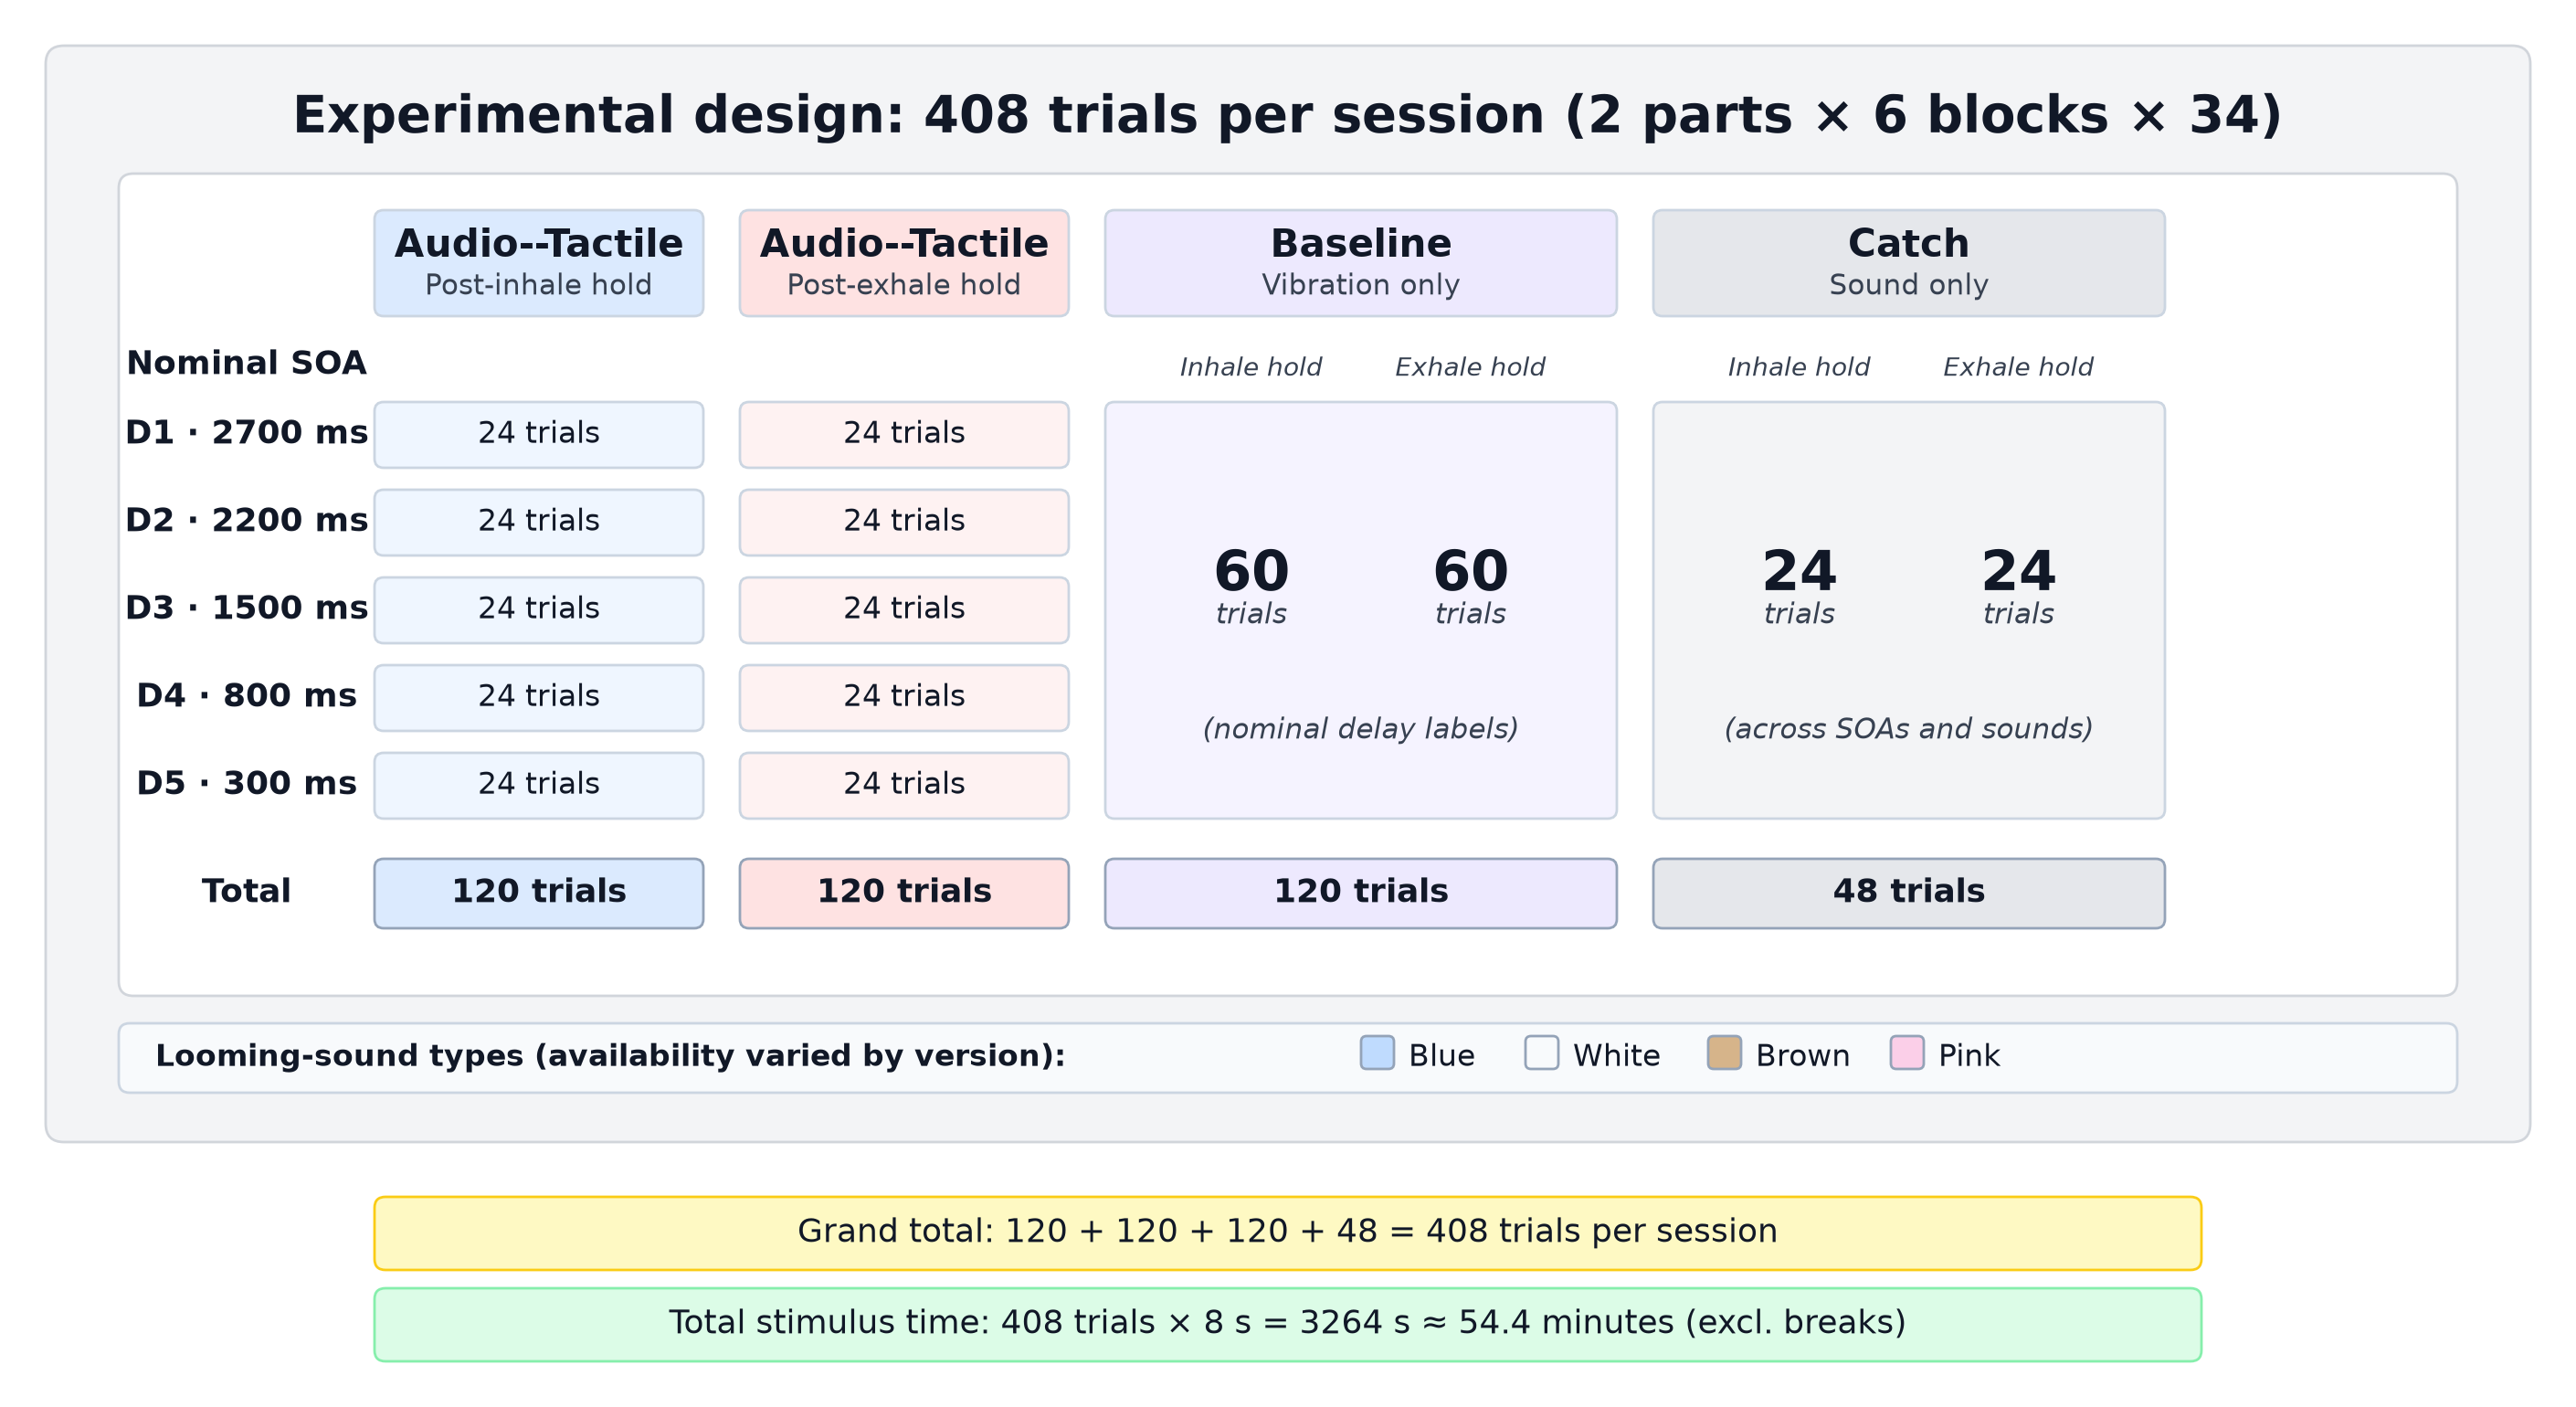
\includegraphics[width=\textwidth]{trial_design.png}
\caption{\textbf{Planned per-session trial distribution across conditions, respiratory phases, and stimulus onset asynchronies.} A full session plans 408 trials, organised as two parts of six blocks (12 blocks of 34). Audio--Tactile trials are distributed evenly across five SOAs (D1--D5; 24 trials per phase $\times$ SOA cell). Available noise types differ by acquisition version. Baseline trials have no auditory SOA or distance; they carry the same five nominal delay labels and are balanced across respiratory phase. Catch trials are balanced across phase and distributed across SOAs and the available noise types.}
\label{study5:fig:trial_design}
\end{figure}

%% ---------------------------------------------------------------------
%% SUBSECTION 4 GOAL
%% Describe stimulus delivery and response capture at run time.
%% Three paragraphs, three ideas:
%%   4a  Playback pipeline and channel routing.
%%   4b  Response capture via a click tone onto the tactile channel.
%%   4c  WASAPI loopback recording of both outputs.
%% The loopback recording is the methodological component that
%% Subsection 5 decodes.
%% ---------------------------------------------------------------------
\subsection{Stimulus delivery and response capture}

%% ---
%% PARAGRAPH 4a GOAL (one idea): how the per-block WAV reaches the
%% participant. Two-channel output, sounddevice callback, WASAPI
%% driver, and the channel-swap that maps file-left to Output 2
%% (Woojer) and file-right to Output 1 (headphones).
%% ---
At run time, each per-block WAV was fully pre-loaded into memory and streamed to the Komplete Audio 6 MK2 on WASAPI via the \texttt{sounddevice} Python binding to the PortAudio library \citep{sounddevice_python}, with a 4096-sample callback block size and a target output latency of 100~ms for stable long-block playback. Python swapped the two channels at the callback boundary so that the left channel of the file was sent to physical Output 2, wired to the Woojer Strap 4 haptic transducer, and the right channel of the file was sent to physical Output 1, wired to the Sennheiser HD 560S headphones. The audio and tactile streams originated from the same file and passed through the same stereo callback, preserving their sample alignment in the digital output stream. Relative acoustic and mechanical onset latencies at the participant were not independently measured.

%% ---
%% PARAGRAPH 4b GOAL (one idea): response capture via click-tone
%% feedback. Each mouse click triggers a short synthetic tone on the
%% tactile channel. The tone is audible to the participant and is
%% what the offline analysis detects, not the OS-level mouse event.
%% ---
Mouse clicks were monitored with the \texttt{pynput} library \citep{pynput_python}, and each click triggered a 1200~Hz, 50~ms synthetic click tone on a separate low-latency \texttt{sounddevice} stream that was routed only to Output 2. The click tone served two purposes. It provided the participant with immediate auditory feedback that the response had registered, and it inserted a detectable event onto the tactile channel that was captured in the loopback recording described below and used for post-hoc reaction-time estimation.

%% ---
%% PARAGRAPH 4c GOAL (one idea): the validated output profile, the
%% continuous WASAPI loopback recording that captures exactly what was
%% sent to the soundcard outputs, and the live event CSV that provides
%% an online behavioural record.
%% ---
Before participant playback, the selected stereo output profile was required to pass a routing preflight in which calibration pulses were sent separately to Output~1 and Output~2 and verified through the corresponding WASAPI loopback endpoint. The documented acquisition profile used the Komplete Audio 6 MK2, with Output~1 assigned to the headphones and Output~2 assigned to the tactile transducer, but the same software could be run on another wired two-channel interface only after the same channel-separation preflight passed. Once participant playback began, the acquisition software was designed to mirror both physical outputs to a WASAPI loopback device and capture them through the \texttt{PyAudioWPatch} extension of the PortAudio interface \citep{pyaudiowpatch}. These source recordings are not presently linked and independently checked for every dataset in the publication pool. Available session WAV files and behavioural CSVs were written to participant-specific data folders with identifying metadata; only coded participant IDs appear in analysis outputs.

%% ---------------------------------------------------------------------
%% SUBSECTION 5 GOAL
%% Describe how the loopback recordings are decoded offline to recover
%% per-trial reaction times. Four paragraphs:
%%   5a  Channel-role inference and tactile-cue detection, plus the
%%       8 s trial grid fit.
%%   5b  Looming onset identification via cross-correlation.
%%   5c  Click-tone detection and RT calculation.
%%   5d  Outcome labelling and alignment to the trial-order CSV.
%% ---------------------------------------------------------------------
\subsection{Reaction-time reconstruction from loopback recordings}

%% ---
%% PARAGRAPH 5a GOAL (one idea): the preprocessing step that turns a
%% continuous loopback recording into a set of per-trial tactile-cue
%% onsets, anchored to an 8 s trial grid. This is the scaffold that
%% every later detection hangs off.
%% ---
For the loopback data to which the waveform-decoding pipeline was applied, reaction times were reconstructed in Python using \texttt{numpy} and \texttt{scipy} \citep{Virtanen2020SciPy}. In that pipeline, audio and tactile channels were identified by the ratio of mean absolute amplitude to root-mean-square amplitude, with the sparser channel assigned as tactile. Tactile cue events were then detected by smoothing the absolute tactile signal with a 10~ms rectangular envelope and thresholding at 0.45 of the envelope peak, subject to a minimum run of 60~ms and a minimum peak amplitude. The resulting cue-onset train was fitted to an 8-second trial grid by jointly minimising the median absolute error between detected onsets and the nominal SOA set, yielding a per-trial cue-onset time in the sample domain of the recorded WAV.

%% ---
%% PARAGRAPH 5b GOAL (one idea): looming onset detection via
%% cross-correlation with the four noise-type templates. This is
%% what lets us label each trial with the noise type actually
%% played and get a second independent anchor for trial timing.
%% ---
For each trial processed by that pipeline, the candidate looming templates for its acquisition version were trimmed to their first 1.5~s of non-silent content, downsampled fivefold for speed, and z-standardised. Each template was cross-correlated with the audio channel of the recording inside the 4.45~s to 7.85~s window relative to the trial origin, using frequency-domain convolution \citep{Virtanen2020SciPy}. The highest-scoring template above threshold assigned the trial its observed noise type and returned the template-onset timestamp, giving an independent anchor for SOA verification where such recording evidence was available.

%% ---
%% PARAGRAPH 5c GOAL (one idea): click-tone detection and RT
%% calculation. The click tone is the actual response event in the
%% recording, and RT is the latency from cue onset to click onset.
%% Emphasises that response timing is measured in the same sample
%% domain as the stimulus.
%% ---
Where the loopback recording and both event markers were available, the 1200~Hz, 50~ms click tone template was z-standardised and cross-correlated with the tactile channel starting at each detected cue onset. Click events were accepted when the local correlation peak exceeded a dynamic threshold of eight median absolute deviations above the local median and were separated from any prior click by at least 100~ms. For such recordings, reaction time was the sample-domain difference between click-tone onset and tactile-cue onset, converted to milliseconds at 44{,}100~Hz. The pooled publication dataset also contains source-recorded reaction times from acquisition versions for which this exact waveform-based definition has not been independently re-harmonised. Consequently the sample-domain timing advantage cannot be assumed for every pooled trial; source-specific timing definitions and verification status are retained in the private provenance crosswalk.

An earlier 40-person source audit catalogued original-recording origins for 31 participants and verified at least one asset hash for each of 17 early-version sessions. That historical audit documented RT-onset variants and unavailable original assets; it is not a new audit of the released 42-person cohort. Source dates, waveform verification status, and acquisition-version identities are deliberately absent from the public tables. The browser companion therefore reports the limits of source-recorded RTs without reconstructing private provenance from arbitrary participant IDs. A file hash establishes source identity, not waveform remeasurement or respiratory-phase accuracy.

%% ---
%% PARAGRAPH 5d GOAL (one idea): outcome labelling and alignment to
%% the per-participant trial-order CSV, producing the analysable
%% dataset. Final sentence returns the reader to the scientific
%% level of abstraction.
%% ---
Trials were labelled against their scheduled trial order and, where available, checked against runtime and recording evidence. Audio--Tactile and Baseline trials with a detected response were labelled hits; Catch trials with a response were false alarms. Unobserved planned slots were kept explicit in the participant audit tables and excluded from reaction-time analysis. Hit-labelled trials without a recorded reaction time contributed to response-quality summaries but not to reaction-time models; missing reaction times were not imputed. The publication-pool analysis table contains only observed planned trials, with trial type, SOA, noise type, scheduled respiratory phase, condition, response outcome, and source-recorded reaction time. Event-marker availability and source location are recorded separately; the analysis table does not imply that every reaction time was newly decoded from a common waveform.

%% ---------------------------------------------------------------------
%% SUBSECTION 6 GOAL
%% Describe how the trial-wise RT table becomes a PPS measure.
%% ---------------------------------------------------------------------
\subsection{Peripersonal-space quantification}

Peripersonal space was operationalised as SOA-dependent audio--tactile reaction time in a looming-sound tactile-detection paradigm \citep{canzoneri2012dynamic, teneggi2013social, noel2015peripersonal}. The tactile pulse occurred at one of five nominal SOAs (300, 800, 1500, 2200, or 2700~ms); longer SOAs corresponded to nearer nominal source positions. The registration labels these SOAs as approximately 100, 73, 50, 27, and 10~cm, although its stated linear 110-to-10~cm, three-second trajectory instead implies approximately 100, 83, 60, 37, and 20~cm at those times. The primary predictor was therefore nominal SOA in milliseconds, not an inferred physical distance. The browser sigmoid implementation retains the registered distance labels for its viability gate; a sensitivity repeated that gate using trajectory-implied positions. It subtracts mean tactile-only Baseline reaction time within each participant $\times$ Condition $\times$ Phase cell: $\mathrm{RT}_{\mathrm{AT}}-\mathrm{RT}_{\mathrm{baseline}}$, with negative values indicating faster Audio--Tactile responses. Baseline trials have no auditory stimulus or acoustic distance. We also compared Audio--Tactile and Baseline RTs at the same nominal SOA label descriptively, without treating the labels as proof of equal cue time. Misses, Catch outcomes, and unobserved planned slots were retained for quality summaries but did not supply reaction times to these curves.

%% ---------------------------------------------------------------------
%% SUBSECTION 6B GOAL
%% Statistical analysis: hierarchical pipeline, sigmoid viability test,
%% model selection, mixed models, ANOVA, contrasts.
%% ---------------------------------------------------------------------
\subsection{Questionnaire scoring and exploratory analysis}

The released participant table contains one set of 37 MAIA-2 items and paired Control/Viscereality spatial-frame-of-reference ratings. The project owner confirmed that MAIA-2 was completed once before the experiment and spatial-frame ratings after each intervention; this timing is supplied by the owner rather than reconstructed from CSV timestamps. MAIA-2 assesses eight self-reported interoceptive dimensions \citep{Mehling2012,Mehling2018}; such reports should be distinguished from objective interoceptive accuracy and metacognitive awareness \citep{Garfinkel2015}. Scores on the administered 0--5 response scale were independently recomputed using the final MAIA-2 item map: Noticing, items 1--4; Not-Distracting, 5--10; Not-Worrying, 11--15; Attention Regulation, 16--22; Emotional Awareness, 23--27; Self-Regulation, 28--31; Body Listening, 32--34; and Trusting, 35--37. Items 5--10, 11, 12 and 15 were reversed as $5-\mathrm{response}$. Each subscale required all constituent items; missing responses were not imputed and no total score was formed. Recomputed and stored means were compared within $10^{-6}$. The release does not supply the administered language record, repeated MAIA scores, or separate body-boundary and small-self fields.

This questionnaire extension is post hoc. Its scoring, estimands and test family were recorded before computing the new associations, but after inspecting the dataset and prior behavioural results. The original registration endpoint returned HTTP 403 during this review; its exact questionnaire wording could not be independently checked. The current repository Methods and analysis contract supply the available account of the plan, with the distinction between registered behavioural questions and this exploratory extension retained. The original registration and administered instrument records require verification before submission.

We reported item frequencies, missingness, subscale descriptives, corrected item--rest correlations and raw Cronbach alpha. Sample-specific reliability can differ by dimension and occasion \citep{Eggart2021}; alpha also has restrictive assumptions \citep{McNeish2018}. We therefore reported pointwise percentile 95\% intervals from 2,000 whole-participant bootstrap draws for means and alpha, without treating a cutoff as evidence of validity, deleting items, or fitting a new 37-item factor structure in this small sample. No clinical change thresholds or pre/post tests were transferred from external validation studies.

Spatial-frame ratings are relevant to experiential changes studied in mindfulness research \citep{hanley_2020}, but the present release includes only condition-labelled A--H responses and corresponding codes 1--8. We verified agreement of these encodings and retained their ordinal order. Category distributions and the full paired transition table were reported. A two-sided exact binomial sign test compared higher versus lower Viscereality ratings among non-ties, with a Clopper--Pearson interval for the higher-rating proportion. Ties remained in the overall paired denominator and in paired dominance, defined as $(n_{\mathrm{higher}}-n_{\mathrm{lower}})/n_{\mathrm{pairs}}$, with a participant-bootstrap interval. Order-stratified counts were descriptive. Equal spacing of categories was not assumed. Because the administered pictogram key is unavailable, higher codes were not labelled allocentric.

The retained supplementary association set comprised 33 Spearman correlations: eight MAIA-2 dimensions with each of Control rating, Viscereality rating, rating-change direction ($-1,0,+1$), and the equal-participant raw-RT Condition $\times$ Phase SOA-slope contrast; plus rating-change direction with that behavioural contrast. The slope contrast used the five cell means and primary SOA scaling; it does not estimate a sigmoid boundary. Complete pairs, average ranks, 19,999 pairing permutations, and the absolute-statistic two-sided tail with the plus-one correction supplied $p$ values. All 33 association $p$ values were reported without multiple-testing correction. This reporting choice replaced the initially specified Holm adjustment after inspecting the results; the analyses remain exploratory. The plus-one rule is part of Monte Carlo permutation inference, not adjustment across tests. Pointwise 95\% intervals used 2,000 paired-person bootstrap draws with re-ranking, excluding and counting undefined draws. Legacy resampling used seed 20261116. These intervals are not simultaneous, and permutation inference assumes exchangeable participants under independence without covariate adjustment. The spatial condition comparison formed a separate, single exploratory test family. Inter-subscale correlations were descriptive without further testing. Missing questionnaires never excluded a person from the primary RT cohort; boundary-related correlations retained the original fit gate.

The main spatial follow-up was subsequently specified as the signed numerical difference $\Delta_i=Y_{i,\mathrm{Viscereality}}-Y_{i,\mathrm{Control}}$, regardless of presentation order. These are two post-intervention ratings, not change from a spatial baseline. This exploratory amendment was recorded before computing the new delta analyses but after inspecting the earlier questionnaire results. All eight continuous MAIA-2 dimensions were correlated separately with numerical $\Delta$ using the same permutation and paired-bootstrap procedure, with an independent generator seeded 20261117. One ancillary correlation linked $\Delta$ to the raw-RT SOA-slope interaction. The eight existing direction-only correlations were retained as ordinal sensitivities; the complete earlier set remained supplementary. Numerical subtraction assumes comparable category steps, and ranking the resulting differences does not eliminate that assumption.

Condition $\times$ pre-experiment MAIA moderation was estimated separately for each dimension by OLS regression of participant $\Delta$ on an intercept and mean-centred MAIA. A second specification added centred presentation order (0=Control-first, 1=Viscereality-first). Differencing eliminates participant intercepts; in this complete two-condition design, the MAIA slope tests the corresponding repeated-measures interaction, while the order coefficient represents Condition $\times$ Order. Independent long-format participant-intercept fits verified the equivalence. Slopes are code steps per one MAIA point. Ordinary two-sided $t$ inference used $n-k$ residual degrees of freedom and interaction $F=t^2$ with $(1,n-k)$ degrees of freedom. This inference assumes a linear conditional mean, independent participants and homoskedastic Gaussian errors. HC3 covariance with $t_{n-k}$ tails supplied approximate heteroskedasticity-sensitive intervals and $p$ values. Both specifications and both uncertainty estimates were reported for every dimension, without multiple-testing correction. Maximum leverage and Cook distance were exported; no participant was removed on these diagnostics. Unknown order excludes a record only from the order sensitivity. Baseline MAIA can moderate the condition contrast; its single pre-experiment measurement cannot mediate an intervention-induced change in MAIA. No mediation analysis was fitted, and order adjustment does not establish absence of carryover.

\subsection{Statistical analysis}
\label{study5:sec:stats}

The analysis plan was registered on AsPredicted (\url{https://aspredicted.org/az9f89.pdf}). The browser implementation follows the registered questions as operationalised in this Methods section, with a fixed executable contract in \texttt{workbook/ANALYSIS\_PLAN.md}. It reads the released 42-person participant and trial tables, preserving the participant as the independent repeated-measures unit. Audio--Tactile and Baseline hits with recorded RT are pooled within person to calculate the mean and sample SD; values within mean $\pm$ 2.5 SD, inclusive, enter RT analyses. Participants with Catch false-alarm rate greater than 30\% are excluded; low hit-rate flags are descriptive. A 200-ms lower cutoff is a sensitivity, not an additional primary rule. The partial session is retained primarily, with explicit exclusion sensitivities. Interactive preparation controls do not change this analysis population.

The primary question uses a Gaussian ML mixed model of individual Audio--Tactile RTs, with Condition, instructed Phase, numeric SOA, all interactions, and a participant random intercept. Control/Viscereality and Exhale/Inhale are coded $-.5/+.5$; SOA is centred and divided by its trial-level sample SD. A likelihood-ratio test compares the full model to the identical model without the three-way term. The secondary model tests Phase $\times$ SOA within Control. Five-level SOA coding is a sensitivity because coding was not fully specified in the registration. Random-intercept ML is profiled exactly using participant sufficient statistics and Woodbury identities, including the zero-variance boundary; it is independently checked against native \texttt{statsmodels} ML fits. Model-based normal Wald intervals condition on estimated covariance parameters and are not small-sample-corrected intervals.

Sensitivities include a participant random SOA slope; linear and log-RT regressions with participant-cluster-robust sandwich covariance; equal-participant contrasts of slopes through five SOA means; complete-person $2\times2\times5$ repeated-measures ANOVA with effect-specific Greenhouse--Geisser correction; condition-order subgroup descriptions; participant-cluster-robust binomial hit-probability regression; and RT regression with within-condition trial position and Condition $\times$ Phase-specific time trends. The random-slope covariance is estimated by Cholesky parameterisation with L-BFGS-B and Powell candidates and a zero-slope boundary. Cluster covariance uses the $G/(G-1)\,(n-1)/(n-p)$ correction and normal Wald inference. The participant-slope sign-flip test uses all sign patterns for at most 16 people and otherwise 19{,}999 Monte Carlo draws with seed 20261015. These analyses probe assumptions rather than replace the primary estimand.

The post hoc missing-RT stress tests assign each hit-labelled Audio--Tactile trial lacking an RT its observed participant $\times$ Condition $\times$ Phase $\times$ SOA cell median. Signed shifts of 0, $\pm100$, and $\pm200$~ms are then applied according to the three-way-contrast direction, and the RT trim and primary model are rerun. These scenarios do not impute misses or identify the missingness mechanism.

The boundary analysis requires trial-level sigmoid $R^2\geq .70$ in all four participant Condition $\times$ Phase cells. The registration did not fully specify the four-parameter form, bounds, trial-versus-mean $R^2$, or whether this exclusion also applied to the raw-RT interaction. We explicitly apply it to boundary inference and report the raw-RT interaction for the roster-based cohort. The transparent reimplementation is $f(x)=a+(b-a)\operatorname{expit}((x-m)/s)$, with $a,b\in[-2000,2000]$~ms, midpoint $m$ within the sampled distance range, and width $s\in[.1,200]$~cm, using three starts. These are disclosed computational choices, not recovered historical optimizer settings. Registered approximate distances and trajectory-implied positions are fitted separately, after subtracting the participant Condition/Phase mean Baseline. Trial objectives use exact SOA sufficient statistics. We additionally calculate the saturated five-SOA trial-level $R^2$ ceiling, which bounds any deterministic SOA curve independently of sigmoid bounds. In-sample sigmoid/linear RMSE, five-mean fits, group fits, and parameter-bound hits are descriptive. Four-parameter fits to five means have one residual degree of freedom and cannot rescue failed trial gates. Boundary midpoint/sharpness and related MAIA-2 or pictographic associations require four qualifying, bound-free trial fits per person; otherwise these outcomes are explicitly not estimable.

A separate post hoc extension examined whether one common procedure could describe four group RT profiles with interpretable sigmoid transitions. Audiotactile and related visuotactile work motivates examining distance-dependent transitions \citep{canzoneri2012dynamic,noel2020rapid}, while expectancy-controlled logarithmic patterns and critical experimental evidence make the response form an empirical question \citep{hobeika2019capturing,holmes2020sounds}. This extension addresses group-profile description; it cannot recover participant boundaries that fail the inference gate. Candidate families were developed after inspecting the data and were not registered. Reporting the full finite grid follows the transparency rationale of multiverse analysis \citep{Steegen2016}, without claiming an exhaustive set of reasonable analyses or treating the most sigmoid-looking result as a confirmatory finding.

Kernel local-constant and local-linear regression provide established signal-smoothing estimators \citep{LiRacine2007}, while local weighted regression, curvature regularization, and isotonic projection provide alternative smooth or shape-constrained approximations \citep{Cleveland1979,Wahba1990,Busing2022}. The four-parameter logistic supplies descriptive location and scale parameters \citep{Ritz2019}; whether the measurements identify them is a separate question from whether the curve fits well \citep{Raue2009}. These sources motivate the estimation tools, not particular bandwidths, bounds, or a requirement that PPS observations follow a sigmoid. The companion's miniature literature review maps each choice to supporting and contrary evidence and records the limits of source access.

The extension used the same retained Audio--Tactile trials and five design positions. Within each participant $\times$ Condition $\times$ Phase $\times$ position cell, five extraction methods were considered: arithmetic mean, median, 10\% and 20\% per-tail trimmed means, and 20\% per-tail winsorized means. Winsorization replaces the lowest and highest $\lfloor .2n\rfloor$ values by the adjacent retained order statistics; it does not remove further trials. The resulting cells were averaged with equal participant weights. Robust summaries probe the influence of extreme RTs and cutoff choices \citep{Ratcliff1993}; the specific percentages remain exploratory. Mean, median and winsorized summaries target different summaries of the response distribution, and the midpoint of a curve through group summaries is not generally the mean of individual midpoints. Thirty-two smoothing specifications crossed Gaussian local-constant and local-linear bandwidths, tricube local-linear bandwidths, discrete curvature penalties, isotonic regression, and Gaussian smoothing followed by isotonic projection, including an unsmoothed comparator. Separate versus common widths across the four curves gave $5\times32\times2=320$ pipelines. Tricube smoothing here is a fixed-bandwidth local-linear implementation without robust residual reweighting; the discrete penalty is not an exact cubic smoothing spline. The complete grid is executable in \texttt{descriptive\_sigmoid.py}.

Distances were normalized to $[0,1]$ using the registered 10--100~cm range. Each candidate fitted $a+A\operatorname{expit}((d-m)/s)$ with $A\in[0,500]$~ms, $m\in[10,100]$~cm and $s\in[4.5,90]$~cm. Increasing RT with distance was imposed as a descriptive shape constraint, allowing $A=0$ rather than forcing a nonzero transition. Offset and amplitude were profiled analytically over 61 equally spaced midpoints and 35 geometrically spaced widths. The selected method used a finer 241-by-81 grid. The width floor prevents transitions substantially narrower than the smallest sampled spacing: its 10--90\% span is 19.8~cm, versus a minimum 17-cm gap. These bounds are explicit regularization choices and were expanded in a sensitivity analysis. No display interpolation was treated as an additional observation.

The same fixed six participant folds (seed 20261016) and five omitted positions evaluated every candidate. For each participant fold and position, extraction, group averaging, smoothing and fitting used only the other participants at the other four positions. The predicted held-out value was centered on the training curve's four unsmoothed extracted values; the fixed scoring target was each test participant's raw cell mean at the omitted position minus that participant's raw mean across the other four positions. Squared errors were averaged over participants, groups and held-out positions. This common shape target permits comparison of mean and robust extraction despite their different overall RT levels. The pipeline with minimum RMSE was selected uniformly for all four curves. Constant and linear benchmarks used identical folds and targets. These reused tuning scores do not constitute an independent post-selection test. Evaluation conditions on profiles cleaned beforehand: participant-wide trimming thresholds use all eligible AT and Baseline hit RTs, including the position later omitted from fitting. Thresholds are not shared across people, but this is not end-to-end prospective prediction with preprocessing learned without the omitted position. The target measures relative profile shape, not absolute RT accuracy.

Uncertainty was described with 1{,}000 participant-cluster bootstrap draws (seed 20261017), retaining all four curves and all five positions together within each sampled person and refitting the selected smoother and logistic model \citep{EfronTibshirani1993}. Within-person extraction is deterministic and can be cached before resampling. Pointwise curve bands include flat fits. Midpoint, width and slope percentile intervals condition on nonflat fits and on the selected method; flat fractions and parameter-bound fractions are reported. Method selection is not repeated within this bootstrap. Paired parameter contrasts use the same resamples and receive no confirmatory $p$ values. Fixed trimmed-mean/kernel alternatives, trajectory-implied coordinates, expanded bounds, and the full candidate table expose method dependence. Subtracting a participant/Condition/Phase constant Baseline would only shift these translation-equivariant curves vertically; no same-label cue-time matching was assumed.

An additional exploratory shape audit required at least the fitted 10--90\% transition within the measured range, two observed positions strictly on each side of the midpoint, one observed position within the 20--80\% transition, and maximum deviation from a best-fitting line on a 181-point display grid of at least 5\% of the model's observed-range change. Positive amplitude was required to classify a transition as visible; flat fits remained allowed. These are explicit post hoc display and sampling criteria, not a validated definition of PPS. The same 320 pipelines were rerun on the restricted grid, and all 160 extraction/smoother combinations were also fitted with a line. Constraints use known design coordinates only, including when a position is omitted; no held-out outcome enters smoothing or fitting. Scores are weighted by the number of test participants, with the same raw-mean contrast target for every family.

To reduce the optimism of reporting a tuning minimum as evaluation evidence \citep{VarmaSimon2006}, six outer participant folds (seed 20261026) each repeated full selection among the candidates of each family using five inner participant folds crossed with five omitted positions. The selected pipeline then predicted outer test participants with each target position omitted from fitting. Inner selection uses all five positions from training participants; this evaluates new people at known design locations, rather than generalization to an unseen experimental design. A zero-contrast constant provides a fourth benchmark. Families and thresholds were developed post hoc, and training sets overlap; no significance test treats folds as independent replicates. Nested evaluation does not remove all sampling variability \citep{Varoquaux2017}; small RMSE differences are interpreted descriptively. The restricted family's final estimates also receive 1{,}000 whole-participant bootstrap refits, conditional on its selected method and constraints. For display, each draw and its corresponding extracted data are centered on the mean across the five sampled positions. Centering is an additive shift and preserves curvature. A separate geometry-only figure normalizes fitted amplitudes, with no observations or uncertainty represented on that scale.

As an independent exploratory check on the observations, raw unsmoothed participant means were projected onto three orthonormal contrasts orthogonal to an intercept and distance. One-sample Hotelling $T^2$ tests assess any nonlinear component, under independent participants, multivariate-normal contrasts and nonsingular covariance. The $F(3,n-3)$ transformation was independently checked against \texttt{statsmodels}; Holm correction covers the four curves. This is not a sigmoid-specific test. The PPS literature motivates investigating distance-dependent transitions \citep{canzoneri2012dynamic,noel2020rapid}, but also reports expectancy-sensitive logarithmic patterns \citep{hobeika2019capturing} and methodological concerns about flexible analysis and small effects \citep{holmes2020sounds}. The focused literature review used indexed abstracts for the PPS and validation papers and official software or author sources for implementation references. Full-paper retrieval and current-literature coverage were limited; the companion records exact searches, access levels and source hashes. No source is taken as evidence that this dataset must be sigmoid.

Supplementary paired contrasts cover Baseline Condition, Phase and their interaction, overall Audio--Tactile-minus-Baseline RT, far-minus-near patterns, same-label Baseline comparisons, and pink-minus-white RT. Their ten unadjusted $p$ values are accompanied by Holm-adjusted values for one family. A four-noise Friedman comparison includes only people with all four sounds available, without assigning acquisition-version labels. Paired contrasts have 95\% $t$ intervals; null detections are not equivalence tests. Same-label Baseline subtraction is descriptive because nominal labels do not establish matched tactile-cue times.

The registration named a Cauchy width of 0.707 but did not fully specify mixed-model priors and comparisons. No BIC approximation is presented as a registered mixed-model Bayes factor. Exploratory one-sample/paired Jeffreys--Zellner--Siow factors use a Cauchy $\sqrt{2}/2$ prior on standardized participant contrasts under a normal likelihood \citep{Rouder2009BayesianT}; Shapiro--Wilk diagnostics accompany them. All data-supported computations run in the browser using NumPy/SciPy in Pyodide, with versions, model status, retained data, and source/input/output hashes in the downloadable record. Source-dependent waveform, respiratory-compliance, date, version, and onset-definition checks are marked unavailable when the public CSVs cannot support them.

%% ---------------------------------------------------------------------
%% SUBSECTION 7 GOAL
%% Brief: respiratory compliance monitoring and participants. One
%% paragraph each.
%% ---------------------------------------------------------------------
\subsection{Respiratory compliance and participants}

%% ---
%% PARAGRAPH GOAL (one idea): clarify that the respiratory belt
%% signal is a compliance check, not an online gating signal, because
%% phase assignment is baked into the WAV structure at generation.
%% ---
Respiratory phase was assigned in the trial schedule under the instructed 4--4--4--4 box-breathing pattern; trials were not gated online by the belt signal. The archived decoder identifies which prerecorded breathing instruction played and can reconstruct final phase labels from trial-order parity. These procedures identify the instructed half-cycle, not the participant's measured inhalation or exhalation. A respiratory belt was part of the acquisition protocol, but the current publication-pool trial table contains protocol phase labels rather than independently belt-verified phases. The available source recordings do not yet support a uniform trial-by-trial respiratory-compliance audit across all four acquisition versions. Phase-related effects must therefore be interpreted as effects of instructed phase under the compliance assumption.

%% ---
%% PARAGRAPH GOAL (one idea): participants. Reports the actual N for
%% the analysed batch and flags the order-condition confound that
%% future counterbalanced data are intended to resolve.
%% ---
The released cohort contains 42 adults aged 19--37 years, with 41 complete sessions and one partial session. Each participant was scheduled for both VR conditions, and 21 completed each condition order. The registration disclosed eight already-collected pilot participants and a stopping target of 30 complete datasets, 15 in each order. The released roster exceeds that target; dates and the reason for continued collection cannot be reconstructed from these public CSVs and require author documentation before submission. A balanced pooled order split does not establish balance within historical acquisition versions. One participant has behavioral PPS measures without the questionnaire battery. The project owner confirmed ethical approval and authorised public release of the deidentified data after removal of names and verification of a separate backup; approval-body details should be supplied by the authors for the final ethics statement.
